%% Template baseado no do Prof. Arnaldo Mandel
%% Veja https://www.ime.usp.br/~am/414/listas/index.html

\documentclass[12pt]{article}

%% Escrevendo em português:

%\usepackage[brazilian]{babel}
\usepackage[utf8]{inputenc}
\usepackage[T1]{fontenc}
\usepackage{textcomp}
\usepackage[T1]{fontenc}
%----------------------------

\setlength{\topmargin}{-.5in}
\setlength{\textheight}{9in}
\setlength{\textwidth}{6.3in}
\setlength{\oddsidemargin}{-.125in}
\setlength{\evensidemargin}{-.125in}

\usepackage[usestackEOL]{stackengine}
\usepackage{xspace}
\usepackage{pifont}
\usepackage{amsmath}
\usepackage{amsfonts}
\usepackage[dvipsnames]{xcolor}
\usepackage{fancybox}
\usepackage{amsthm}
\usepackage{listings}
\usepackage{hyperref}
\usepackage{todonotes}

\usepackage{MnSymbol,wasysym}
\usepackage{marvosym}

\pagestyle{empty}

\definecolor{darkgreen}{RGB}{0, 133, 117}
\definecolor{yelloworange}{HTML}{FAA21A}

\newcommand{\N}{{\tt I\kern-.2em N \relax}}      % N        |N
\def\pule{\vspace{0.2cm}}
\def\pulao{\vspace{0.5cm}}
\def\pulaozao{\vspace{1cm}}
\def\ni{\noindent}

\newcommand{\Si}{\ensuremath{\Sigma}\xspace}
\newcommand{\Sis}{\ensuremath{\Sigma^*}\xspace}
\newcommand{\Ga}{\ensuremath{\Gamma}\xspace}
\newcommand{\Gas}{\ensuremath{\Gamma^*}\xspace}
\newcommand{\serio}{\ding{98}\xspace}
\newcommand{\LP}{L\&P\xspace}
\newcommand{\conj}[2]{\ensuremath{\{#1\,|\;#2\}}}
\DeclareMathOperator{\Ima}{Im}
\newcommand{\ssq}{\ensuremath{\subseteq}\xspace}
\newcommand{\union}{\mathop{\bigcup}\displaylimits}
\newcommand{\Rfield}[1]{\ensuremath{\mathbb{R}^{#1}}\xspace}
\newcommand{\del}{\ensuremath{\text{d}}\xspace}
\newcommand{\expct}[1]{\ensuremath{\langle {#1} \rangle}\xspace}

\begin{document}

\newtheorem{theorem}{Teorema}%[section]
\newtheorem{corollary}{Corolário}[theorem]
\newtheorem{lemma}[theorem]{Lema}

\begin{center}
\Huge \bf
Parallelizing GCC with Threads
\vspace{0.5cm}
\end{center}
\vspace*{\fill}
{
     \centering
     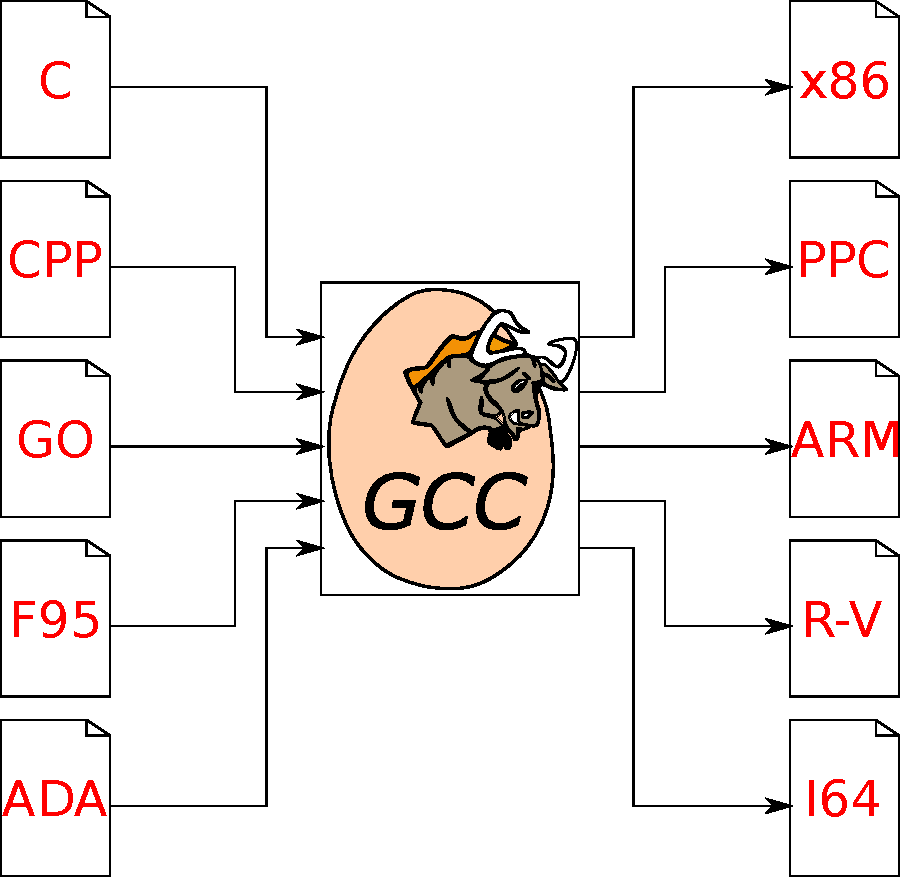
\includegraphics[scale=0.7]{logo.pdf}
    \par
}
\vspace*{\fill}
\normalsize{
\noindent\textcolor{darkgreen}{Giuliano Belinassi} \\
University of São Paulo -- Brazil \\
IRC: giulianob in \#gcc \\
Email: \href{mailto:giuliano.belinassi@usp.br}{\texttt{giuliano.belinassi@usp.br}} \\
Github: \url{https://github.com/giulianobelinassi/} \\
Date: \today
}
\newpage

\begin{section}{About Me}
    Currently pursuing a Master's Degree in Computer Science at the University
    of São Paulo with a Computer Science Bachelor's degree in the same
    institution. I've always been fascinated by topics such as
    High-Performance Computing and Code Optimization, having worked with
    a parallel implementation of a Boundary Elements Method software in GPU,
    and I am currently
    conducting research in compiler parallelization. Therefore, I am applying
    to the GNU Compiler Collections
    (GCC) both as a research project in parallelization of compilers, and
    mainly to become a part of the free software community.

    \textbf{Skills}: Strong knowledge in C, Concurrency, Shared Memory Parallelism, Vim, and command line utilities (grep, sed, ...)
\end{section}

\begin{subsection}{Contributions to GCC}

I've submitted some patches, mainly adding inline optimizations to
trigonometric functions. These kind of patches requires deep testing to guarantee
that the optimization did not yield severely incorrect results, which
concluded in a blog post about the patch \textit{Optimize $\sin (\arctan (x))$}
\footnote{https://flusp.ime.usp.br/updates/2019/03/26/making-gcc-optimize-some-trigonometric-functions/}.
I did this blog post both to register how to add these new kinds of optimizations,
and also to encourage newcomers to contribute to GCC.

\begin{table}[!htbp]
\centering
\begin{tabular}{|l|l|}
\hline
Name                                                                                      & Status   \\ \hline
    \href{https://patchwork.ozlabs.org/patch/981596/}{Optimize $\sin (\arctan (x))$}      & \color{darkgreen}{\texttt{Accepted}} \\ \hline
    \href{https://patchwork.ozlabs.org/patch/1003988/}{Optimize $\sinh (\text{arctanh} (x))$}   & \color{darkgreen}{\texttt{Accepted}} \\ \hline
    \href{https://patchwork.ozlabs.org/patch/961362/}{Fix typo 'exapnded'}                & \color{darkgreen}{\texttt{Accepted}} \\ \hline
    \href{https://en.wikibooks.org/wiki/LaTeX/Hyperlinks}{Split 'opt and gen' variable}   & \color{yelloworange}{\texttt{Working}} \\ \hline
    \href{https://patchwork.ozlabs.org/patch/1023211/}{Update $\sin (\arctan (x))$ test}  & \color{yelloworange}{\texttt{Waiting Stage1}} \\ \hline
    \href{https://patchwork.ozlabs.org/patch/1046302/}{Fix PR89437}                           & Wilco Dijkstra version accepted \\ \hline
\end{tabular}
\end{table}

\end{subsection}

\begin{section}{Parallelization Project}
While looking for topics in compiler's field that touched subjects that I
am interested in for the subject of my master's thesis, I found this
parallelization project in GSoC 2018. With this in mind, I started a
discussion in the mailing list to understand what this project is about,
which was parallelizing the GCC internals to be able to compile big files
faster, which got my
interest\footnote{\url{https://gcc.gnu.org/ml/gcc/2018-11/msg00073.html}}.
This was way before the list of GSoC accepted organizations.

As stated in PR84402\footnote{\url{https://gcc.gnu.org/bugzilla/show\_bug.cgi?id=84402}},
there is a parallelism bottleneck in GCC concerning huge files, with hundreds of
thousands of lines of code. In the course of the discussion,
Bin Cheng\footnote{\url{https://gcc.gnu.org/ml/gcc/2018-12/msg00079.html}}
reported that
he is facing a similar issue with his project, stating that parallelizing the
compiler may solve his problem. These topics supports the interest in the
community for this project.

\end{section}

\begin{subsection}{Current Status}
in PR84402, Martin Liška posted a graphic showing the existence of
parallelism bottleneck in GCC compilation due to huge files such as
\texttt{gimple-match.c} in a 128-cores machine. He also posted a amazing patch to
GNU Make to collect the data and a script to plot the graphic, which I used
to reproduce the same behaviour in a 64-cores machine that is available in
my university.

Unfortunately, I found this approach not easy to reproduce, as
it requires compiling and installing a custom version of Make, generated
gigabytes of data which requires parsing by a script that often crashed due
to a very large SVG. With this in mind, I created a set of
tools\footnote{\url{https://github.com/giulianobelinassi/gcc-timer-analysis}}
using a complete distinct approach, generating less data, is more stable, and
plotted better graphics, such as the one in Figure \ref{fig:analysis}.

I also explored the GCC codebase in order to find the performance bottleneck for
such huge files. Analyzing the most time-consuming file in GCC's project
(\texttt{gimple-match.c}), I found that the method
\texttt{finalize\_compilation\_unit} of
class \texttt{symbol\_table} takes around 50s to compile with a
\texttt{--disable-checking} GCC under \texttt{-O2}, with the \texttt{expand\_all\_functions}
routine taking most of this time. Currently, my strategy is to try to parallelize
this part of the compilation, as it seems possible because I've already made GCC output
functions in reverse orders.

Furthermore, I am also studying the theoretical background behind \texttt{GIMPLE},
    and \texttt{cgraphs}. I have read the \texttt{GIMPLE}
documentation\footnote{\url{https://gcc.gnu.org/onlinedocs/gccint/}}, and
I am looking for how \texttt{cgraph} works internally, both in theory and in
GCC.

\end{subsection}

\begin{subsection}{Planned Tasks}
    Currently, my plan consists in three high-level topics, but more details
will be provided as I proceed into the project. These topics are:

\begin{enumerate}
    \item \textit{Document the global variables and states}. The \texttt{cgraph}
clearly was not implemented with this kind of parallelism in mind, as it has a lot
of global states (i.e., RTL initialization, possible node dependency,
Garbage Collector, ...). This has to be rewritten into something that could
be handled locally for each thread, or insert locks.
	\item \textit{Develop a parallel prototype}. GCC supports a lot of systems
with different threading schemes. Discussion in the mailing list suggested the
use of pthreads and C++11 threads, however, this may not be the easiest way to
develop parallel software and I may use OpenMP to accelerate the development.
	\item \textit{Refactor the parallel prototype}. Here the aim is to improve
the previous implementation with proper cross-platform support, and remove any
OpenMP code.
\end{enumerate}


\begin{figure}[ht]
 \centering
 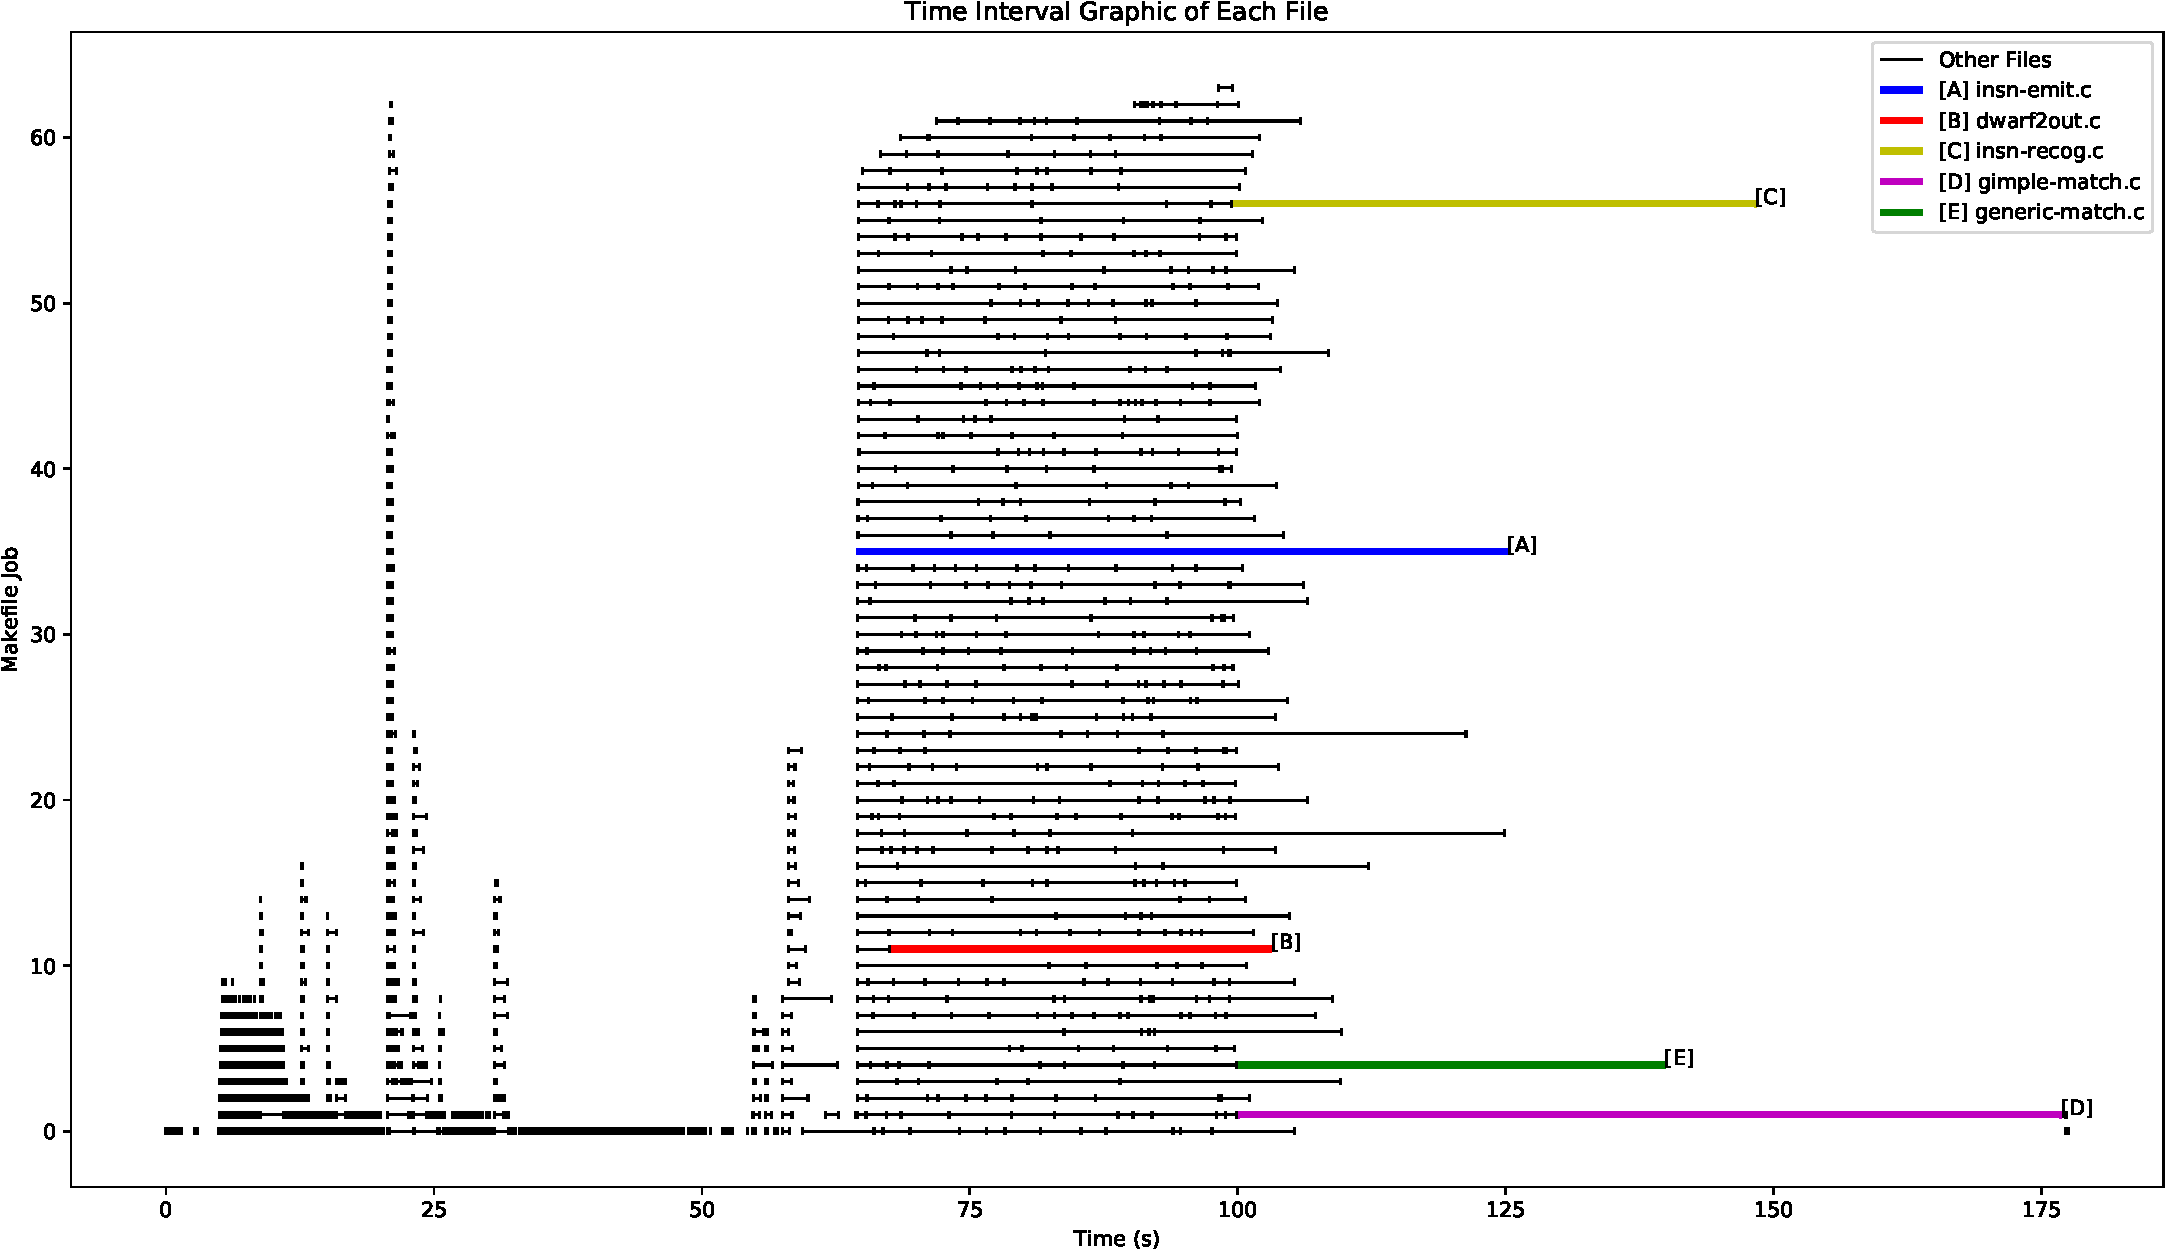
\includegraphics[scale=0.6, angle=-90]{out-crop.pdf}
 \caption{Elapsed time analysis in GCC compilation for a 64 cores machine, No bootstrap}
 \label{fig:analysis}
\end{figure}

\end{subsection}

\end{document}
